\chapter{Implementacja prototypu systemu}
\label{cha:ImplementacjaPrototypu}

Ten rozdział poświęcony jest szczegółom związanym z implementacją prototypu systemu. Była to najbardziej pracochłonna część pracy. Celem implementacji systemu jest sprawdzenie działania technologi jaką jest Adobe P2P Multicasting. Czy rozwiązanie to nadaje się dla projektowanego ,,Społecznościowego, internetowego systemu monitoringu''.

\section{Co zostało zaimplementowane}
Prototyp systemu dostępny jest on-line pod adresem \url{http://facewithme.com}. Przy tworzeniu prototypu systemu skupiono się na pięciu elementach systemu (szczegóły architektury znajdują się \namedref{sec:EtapIwstepnaArchitekturaSystemu}):

\begin{packed_item}
    \item{Interfejs WWW}
    \item{Baza danych}
    \item{Serwer RTMFP}
    \item{Mobile Broadcaster}
    \item{Browser Receiver}
\end{packed_item}

Dzięki wybraniu ww. elementów udało się stworzyć system zdolny do przetestowania transmisji wideo pomiędzy Mobile Broadcaster, a Browser Receiver, za pomocą technologii Adobe P2P Multicast. Interfejs WWW umożliwia dodatkowo ładną prezentację oraz wyszukiwanie streamów w zadanej lokalizacji czy też personalizację ustawień.

\newpage
Na poniższym rysunku widać architekturę  zaimplementowanej częsciu systemu wraz z prezentacją transmisji P2P. Należy zwrócić uwagę, że Serwer RTMFP nie bierze czynnego udziału w transmisji wideo, służy jedynie do rozgłaszania klientów udostępniających stream. Transmisja wideo odbywa się pomiędzy Mobile Broadcasterem, a klientami Browser Receivera.
\begin{center}
    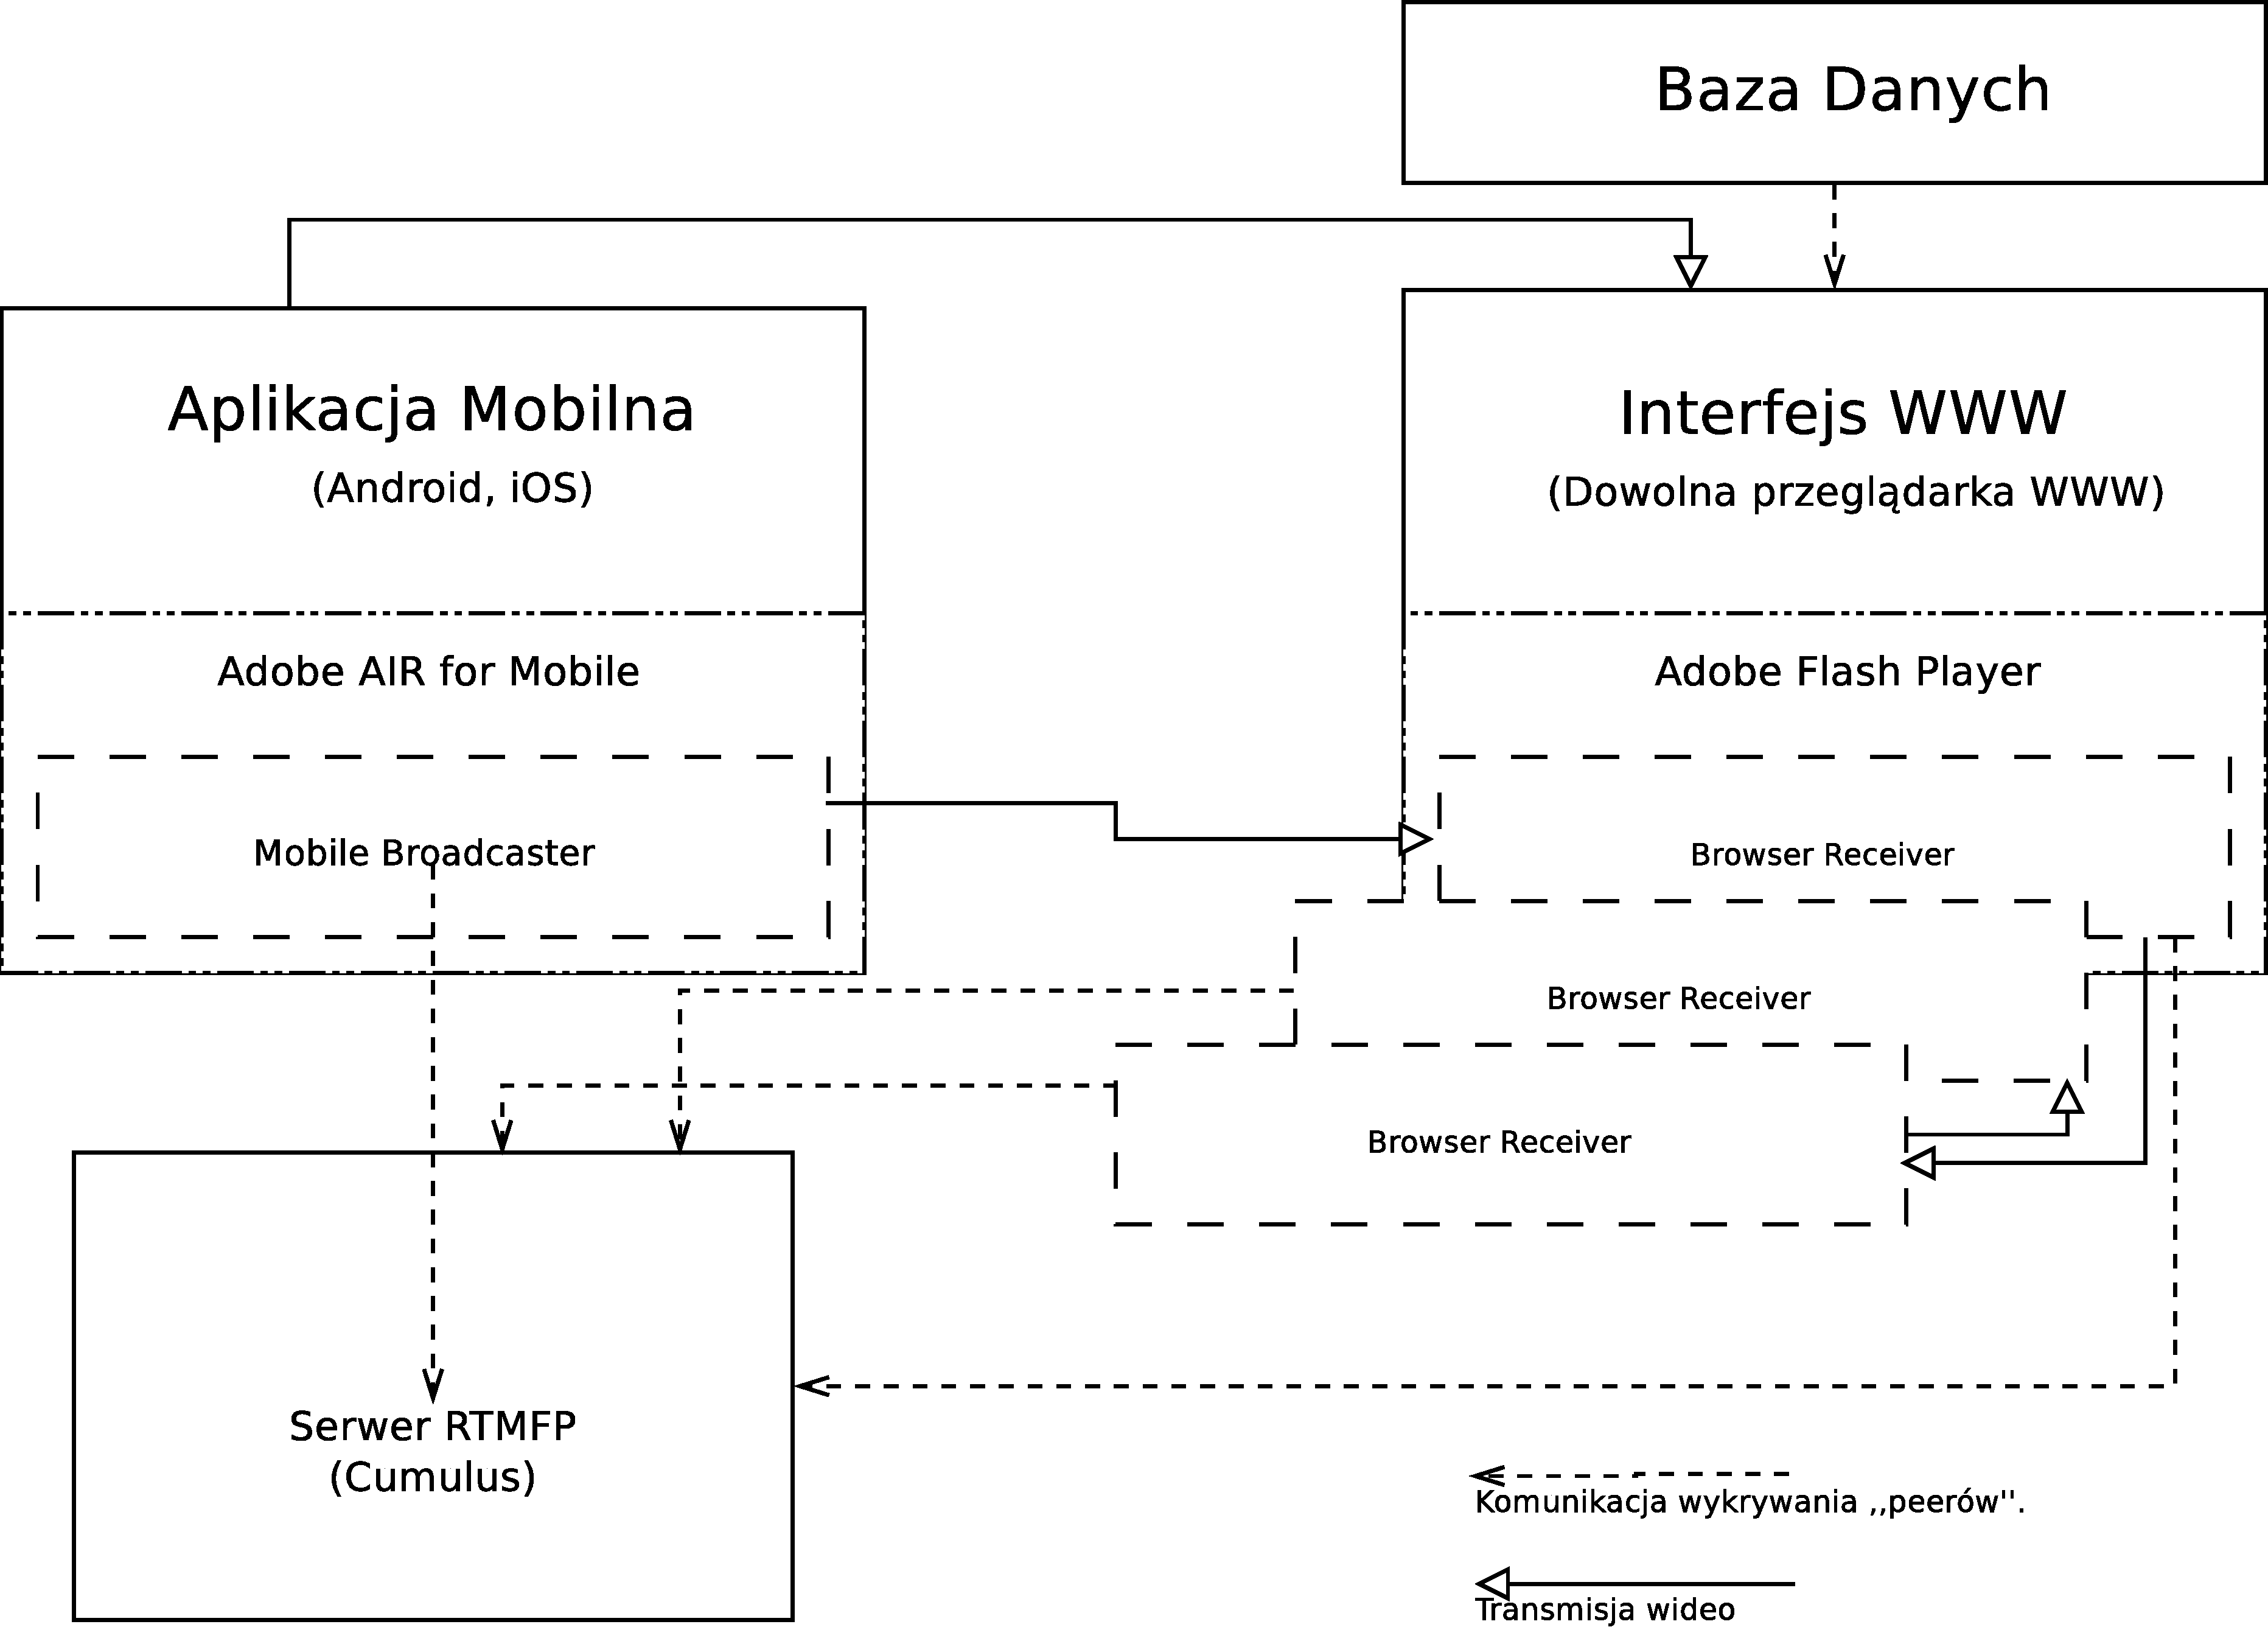
\includegraphics[width=\textwidth]{diagramy/architektura-implementacja.pdf}
    \captionof{figure}{Architektura implementacji prototypu systemu uwzględniająca transmisję wideo z Mobile Broadcastera do kilku Browser Receiverów.}
    \label{fig:architekturaImplementacji}
\end{center}

\subsection{Interfejs WWW}
Niżej przedstawiono elementy, które udało się zaimplementować w części systemu nazwanej Interfejs WWW. Szczegóły i opis architektury znajdują się \namedref{sec:EtapIwstepnaArchitekturaSystemu}.

\begin{packed_item}
    \item{System rejestracji użytkownika (\url{http://facewithme.com/accounts/register}), można zobaczyć na rysunku \ref{fig:rejestracja}.}
    \item{System logowania użytkownika (\url{http://facewithme.com/accounts/login}), można zobaczyć na rysunku \ref{fig:logowanie}.}
    \item{Panel administracyjny do zarządzania streamami, kategoriami i użytkownikami (\url{http://facewithme.com/admin}), można zobaczyć na rysunku \ref{fig:panelAdministracyjny}.}
    \item{Interaktywną mapę prezentującą streamy (\url{http://facewithme.com}), można zobaczyć na rysunku \ref{fig:interaktywnaMapa}.}
    \item{Funkcję automatycznej lokalizacji użytkownika i ustawienie pozycji mapy zgodnie z nią (\url{http://facewithme.com}), można zobaczyć na rysunku \ref{fig:interaktywnaMapa}.}
    \item{Listowanie wszystkich streamów nadawanych w systemie z podziałem na kategorie (\url{http://facewithme.com/stream/list}), można zobaczyć na rysunku \ref{fig:listaStreamow}.}
    \item{Wyświetlanie Browser Receivera, można zobaczyć na rysunku \ref{fig:browserReceiver}.}
\end{packed_item}

\begin{center}
    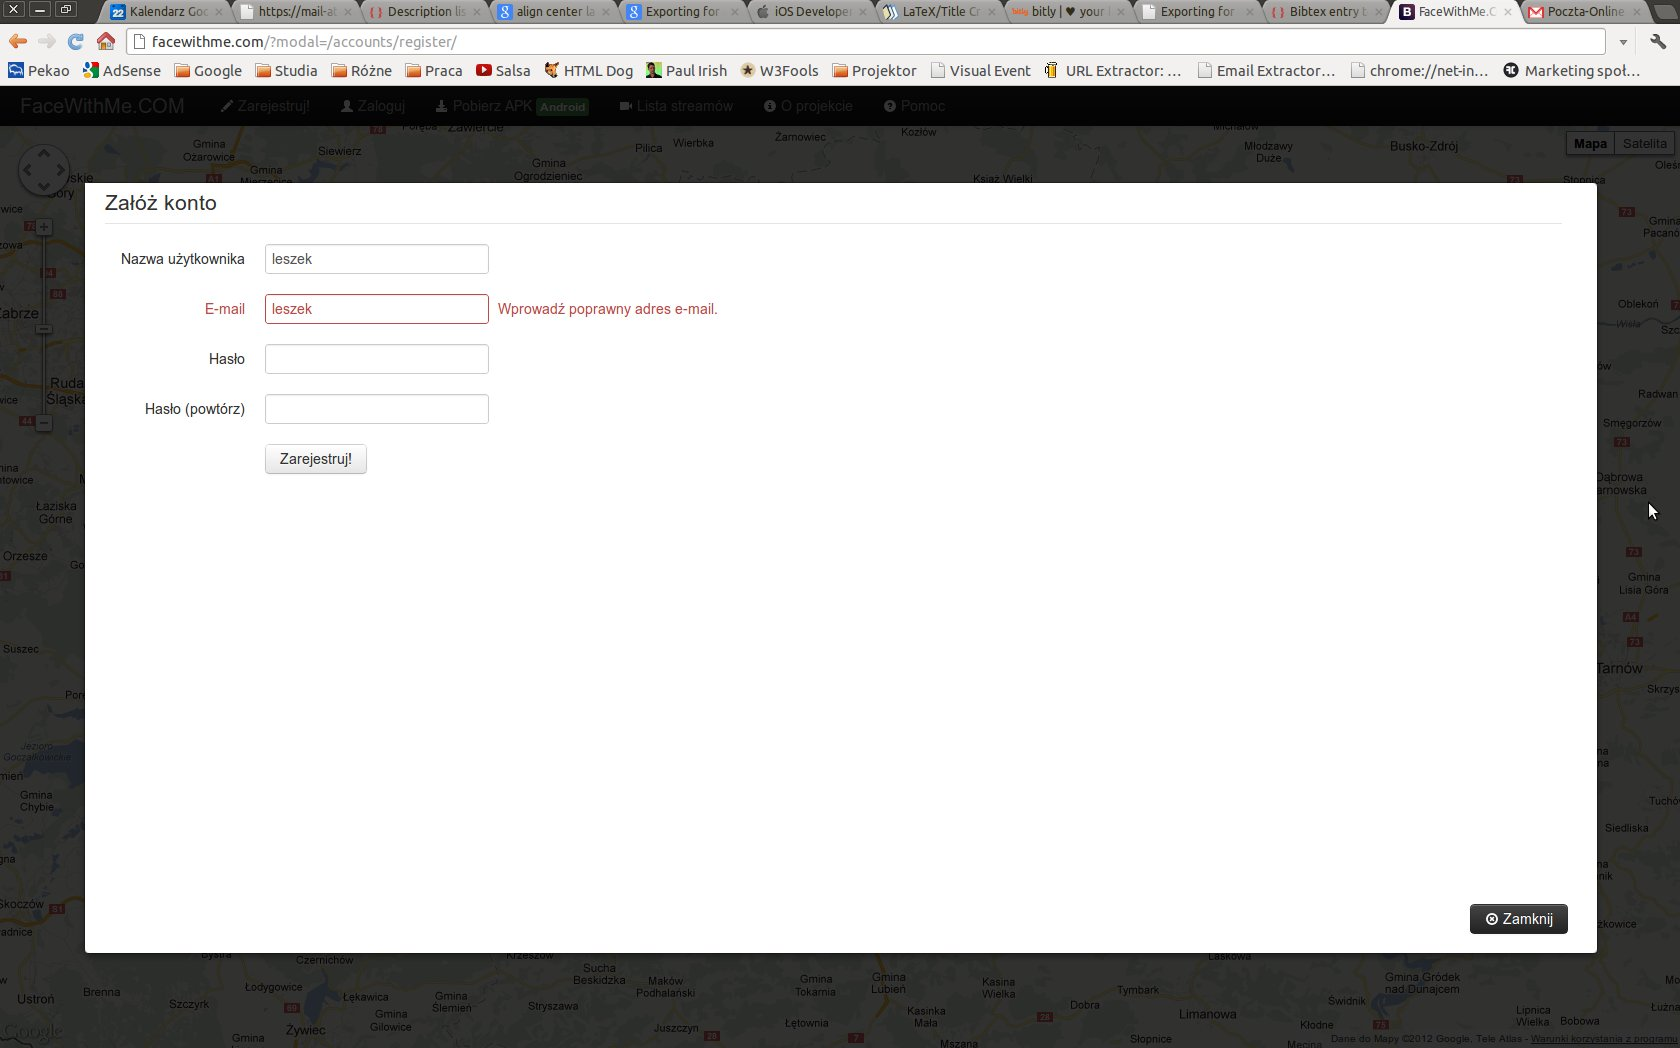
\includegraphics[width=\textwidth]{img/screens/interfejs_www/rejestracja.jpg}
    \captionof{figure}{System rejestracji użytkownika.}
    \label{fig:rejestracja}
\end{center}
\begin{center}
    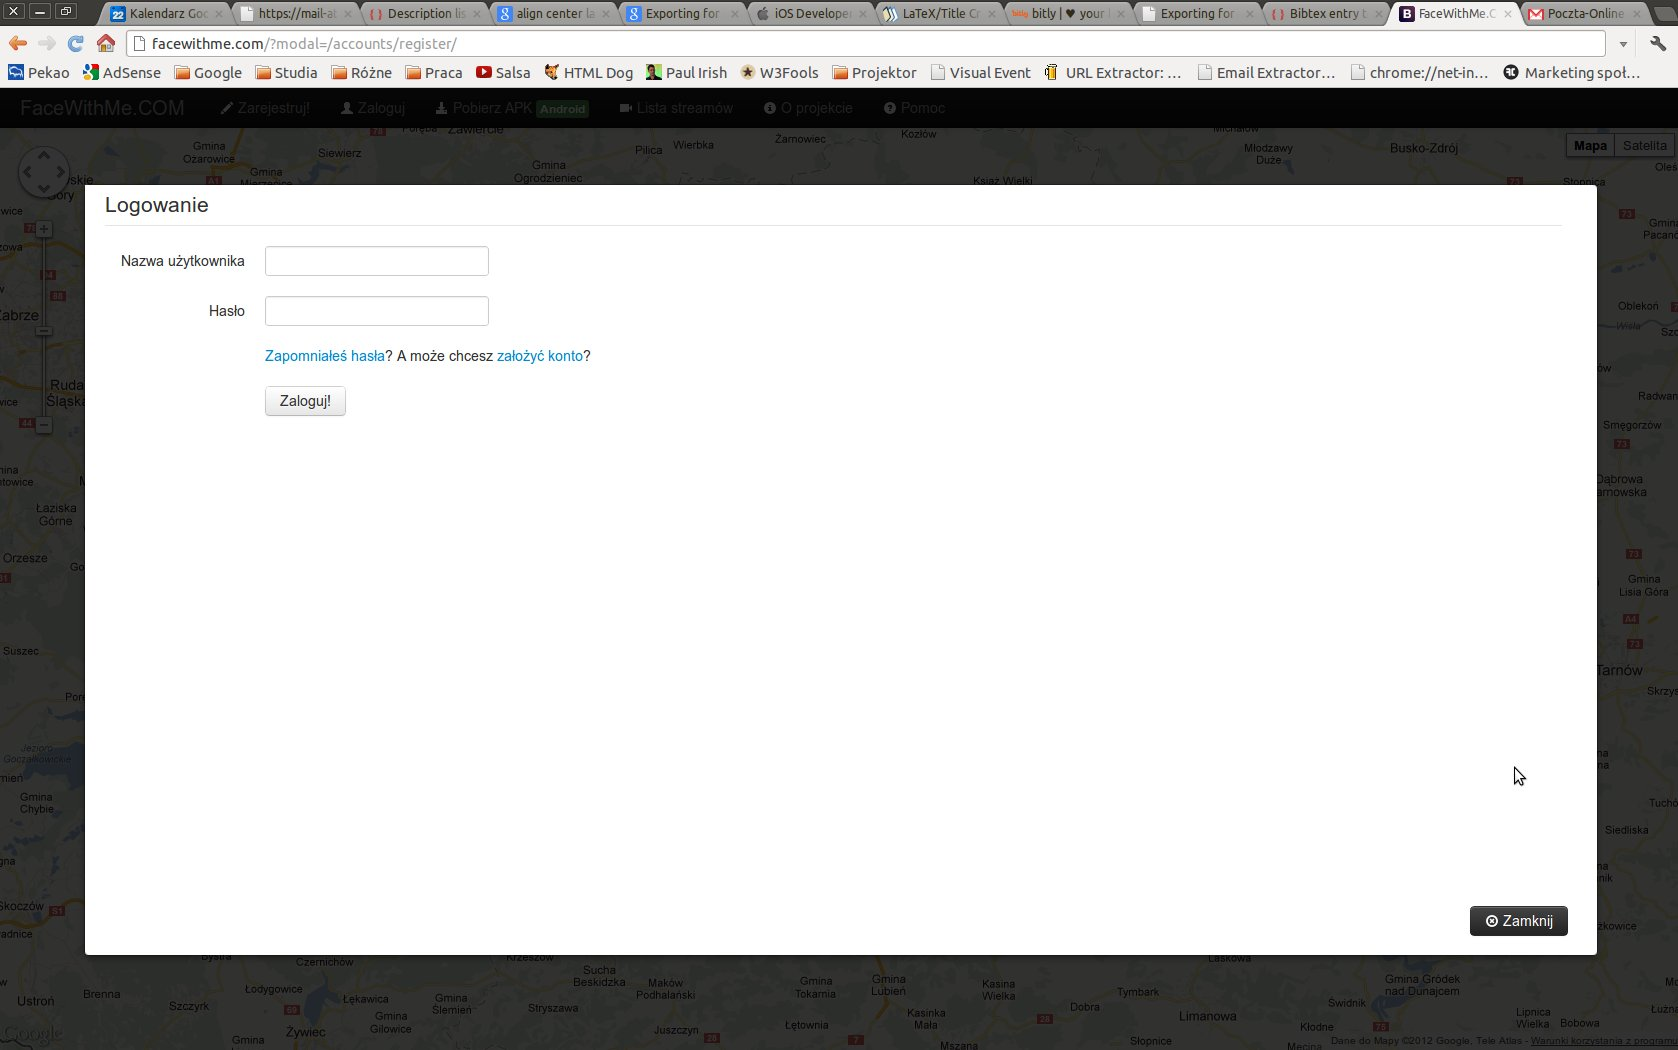
\includegraphics[width=\textwidth]{img/screens/interfejs_www/logowanie.jpg}
    \captionof{figure}{System logowania użytkownika.}
    \label{fig:logowanie}
\end{center}
\begin{center}
    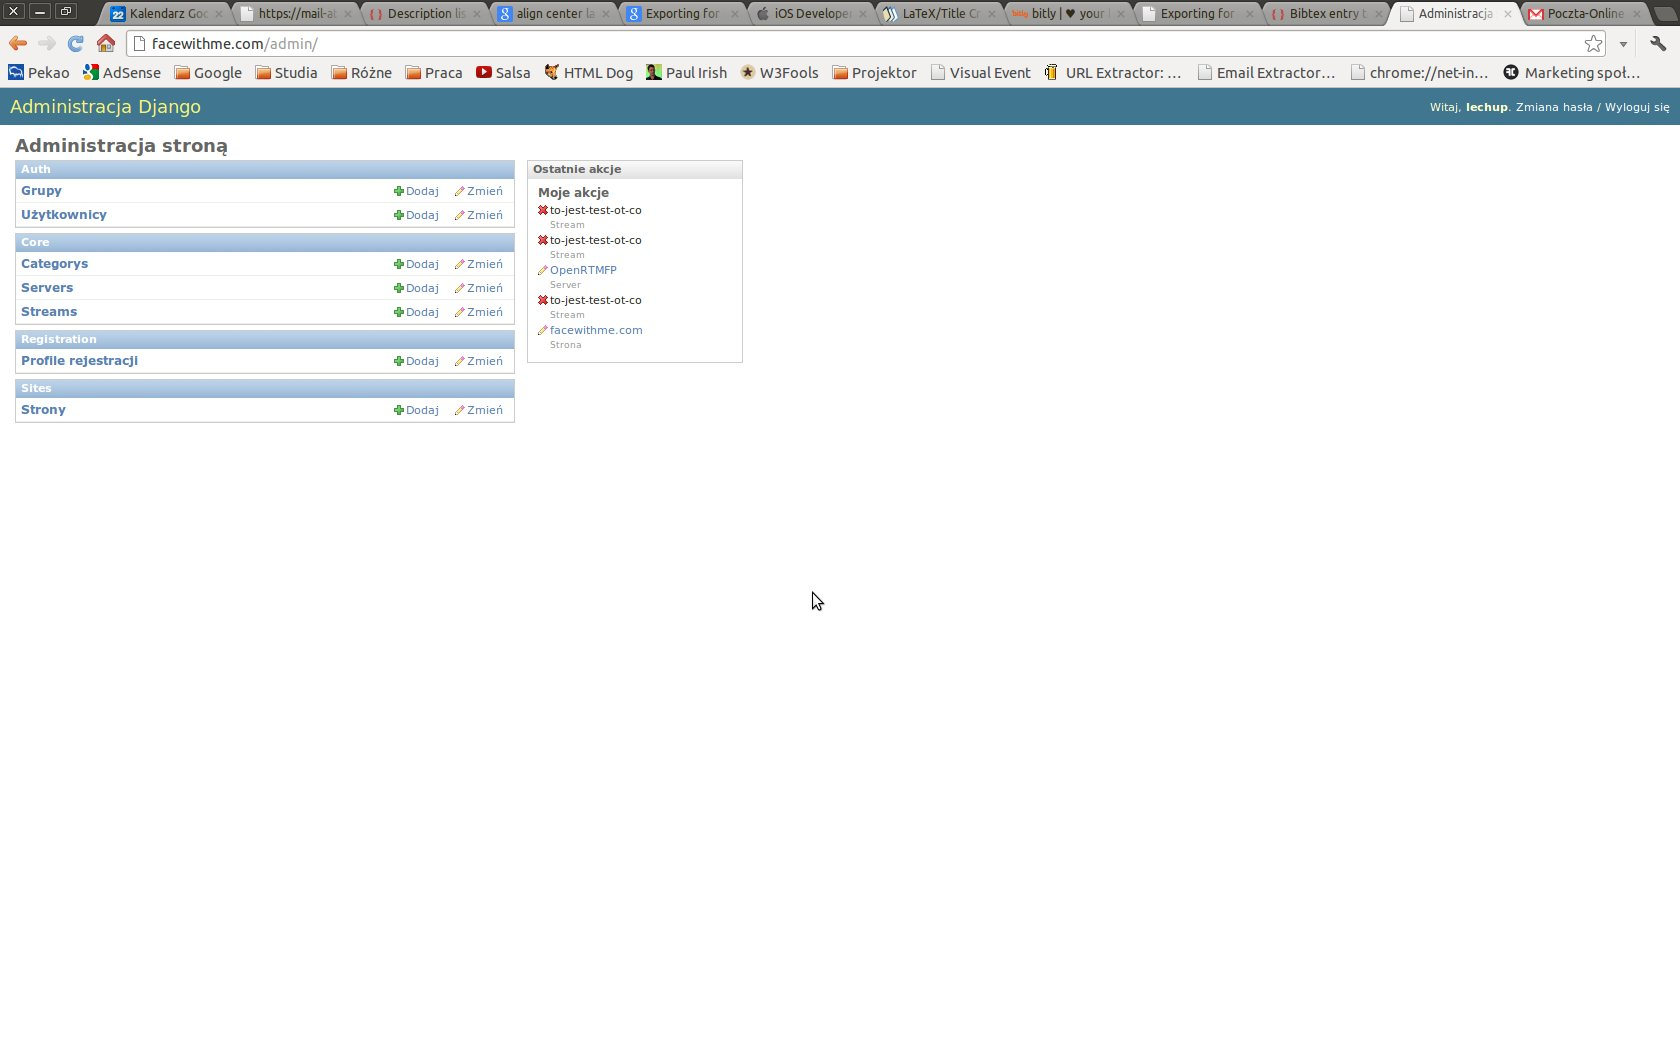
\includegraphics[width=\textwidth]{img/screens/interfejs_www/panel-administracyjny.jpg}
    \captionof{figure}{Panel administracyjny do zarządzania streamami, kategoriami i użytkownikami.}
    \label{fig:panelAdministracyjny}
\end{center}
\begin{center}
    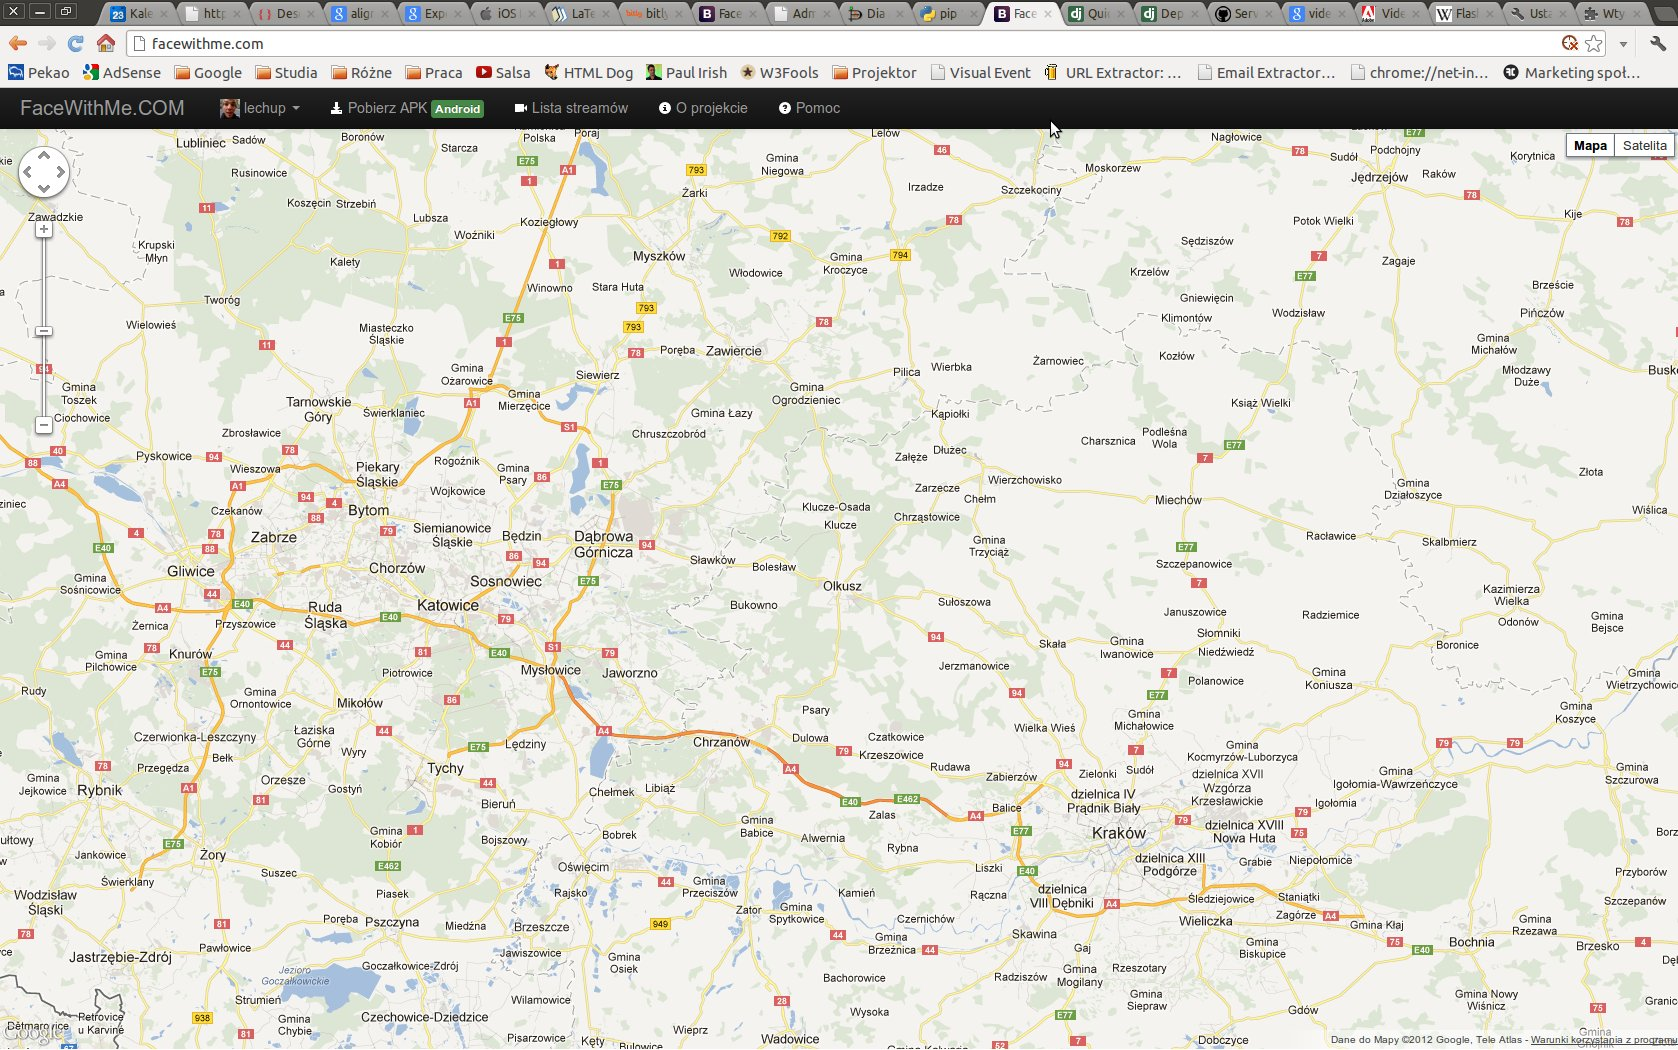
\includegraphics[width=\textwidth]{img/screens/interfejs_www/interaktywna-mapa.jpg}
    \captionof{figure}{Interaktywna mapa prezentująca streamy.}
    \label{fig:interaktywnaMapa}
\end{center}
\begin{center}
    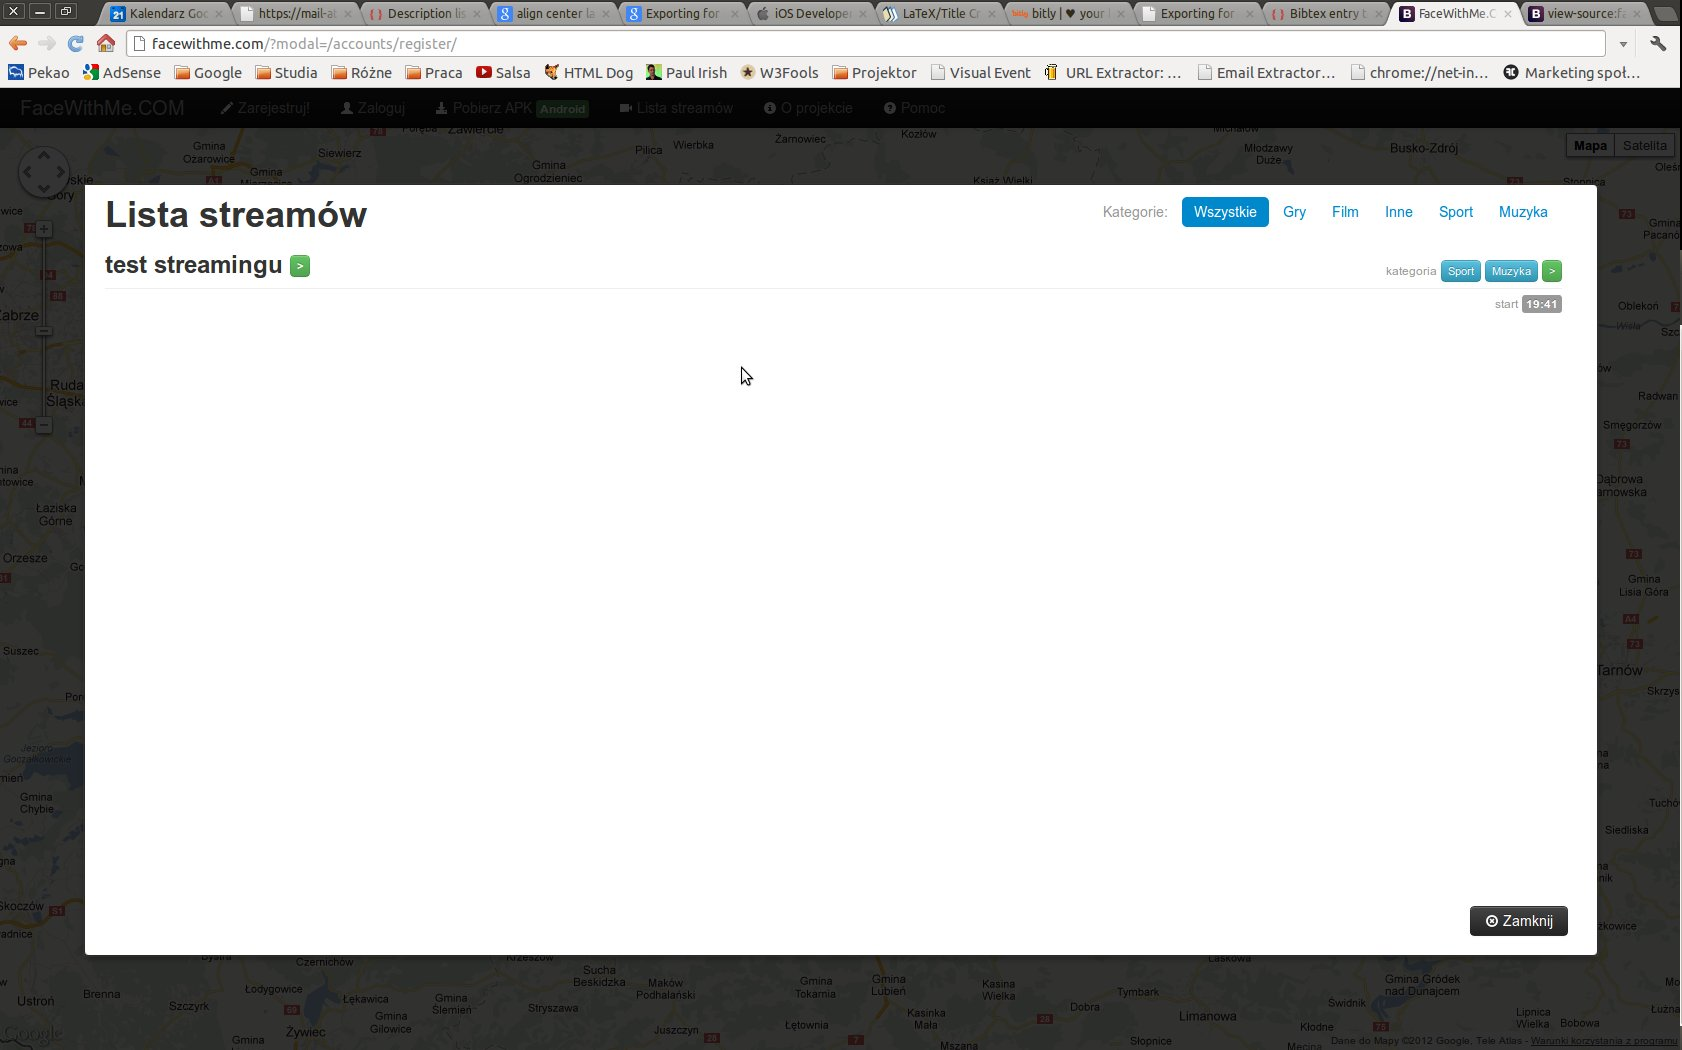
\includegraphics[width=\textwidth]{img/screens/interfejs_www/lista-streamow.jpg}
    \captionof{figure}{Lista streamów nadawanych w systemie z podziałem na kategorie.}
    \label{fig:listaStreamow}
\end{center}
\begin{center}
    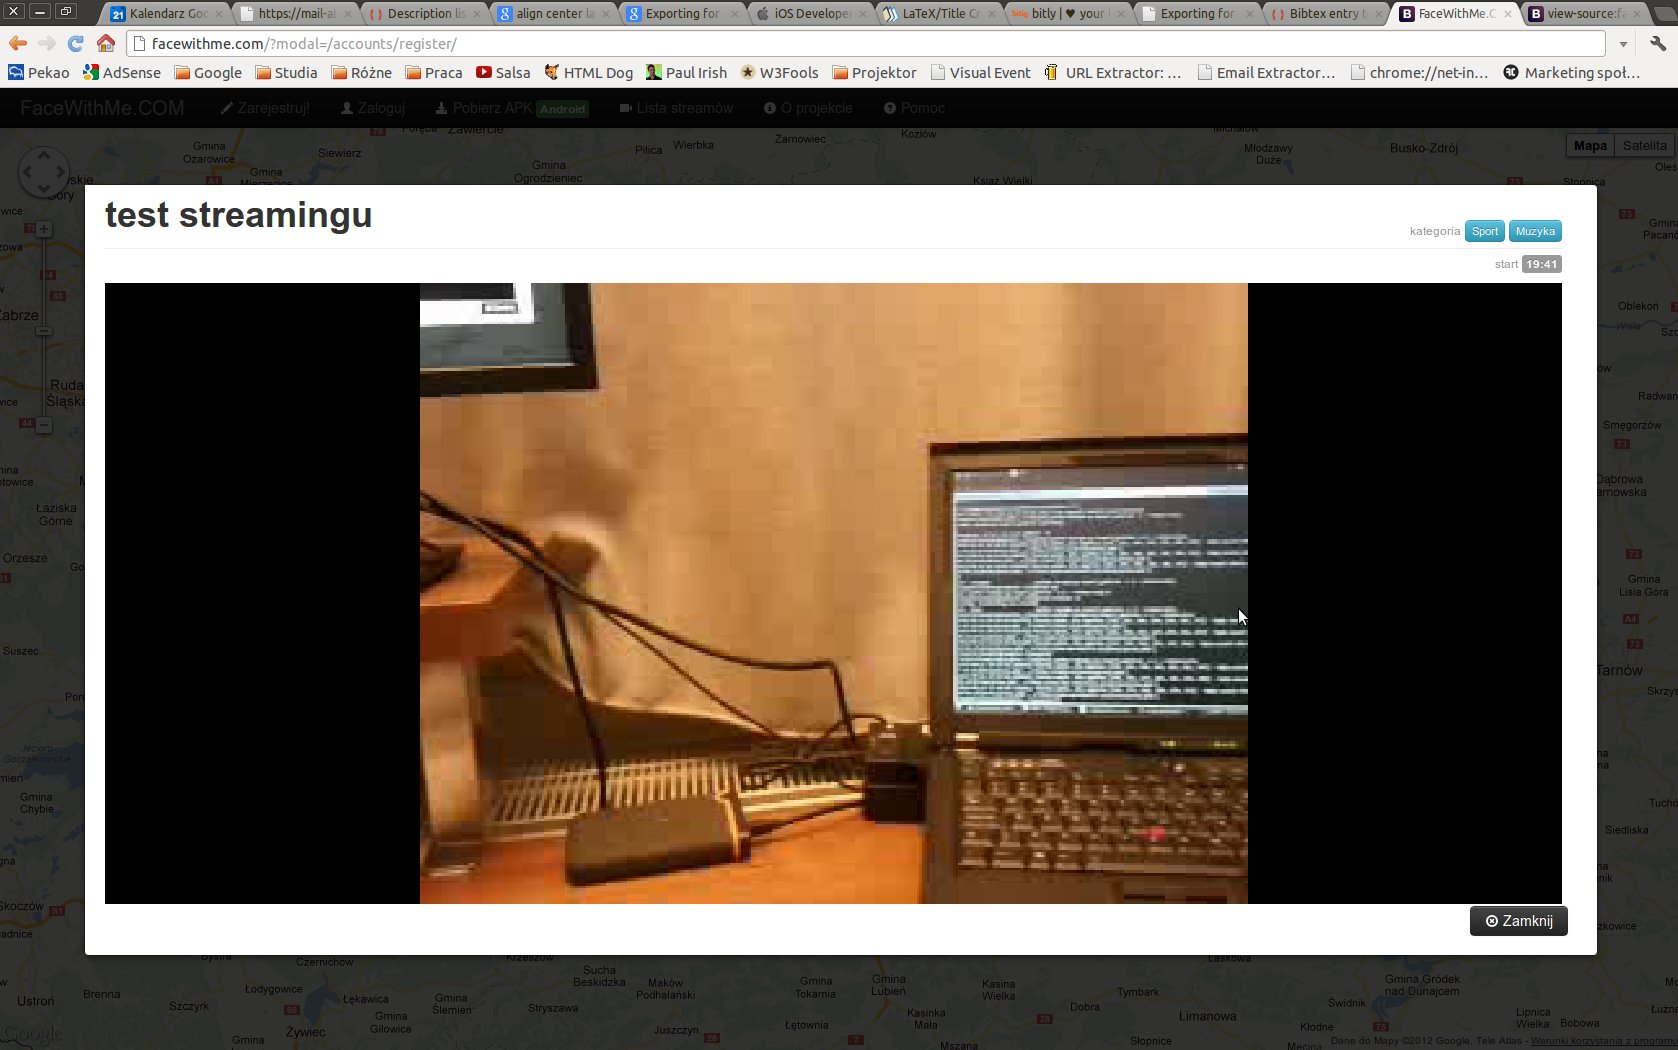
\includegraphics[width=\textwidth]{img/screens/interfejs_www/browser-receiver.jpg}
    \captionof{figure}{Wyświetlanie Browser Receivera w Google Chrome.}
    \label{fig:browserReceiver}
\end{center}


\newpage
\subsection{Mobile Broadcaster}
Mobile Broadcaster, czyli aplikacja umożliwiająca nadawanie streamu -- szczegóły \namedref{sec:EtapIwstepnaArchitekturaSystemu} -- jest aplikacją na systemy Android wykonana w środowisku AIR. Na przygotowanej stronie \url{http://facewithme.com} można pobrać aplikację. Aplikacji nie umieszczono w Google Play, gdyż nie jest ona produktem skończonym, a tylko takie można umieszczać na tej platformie. Aplikacja w formie instalatora na systemy Android została umieszczona również na dołączonej płycie CD w katalogu \texttt{./src/Django/facewithme/apps/core/static/FaceWithMe.apk}. Aplikacja została przetestowana z wykorzystaniem środowisk uściślonych w \namedref{sec:EtapIprzeprowadzoneTesty}. Niżej przedstawiono funkcje Mobile Broadcastera, które udało się zaimplementować w prototypie systemu.

\begin{packed_item}
    \item{Panel udostępniania streamu wideo, można zobaczyć na rysunku~\ref{fig:MB1}.}
    \item{Streaming wideo, można zobaczyć na rysunku~\ref{fig:MB2}.}
    \item{Ustawianie jakości streamu w trakcie nadawania, można zobaczyć na rysunku~\ref{fig:MB3}.}
    \item{Panel ustawień aplikacji, można zobaczyć na rysunku~\ref{fig:MB4}.}
    \item{Panel DEBUG aplikacji, można zobaczyć na rysunku~\ref{fig:MB5}.}
\end{packed_item}

\begin{figure}[h]
    \centering
    \begin{subfigure}{0.4\textwidth}
        \centering
        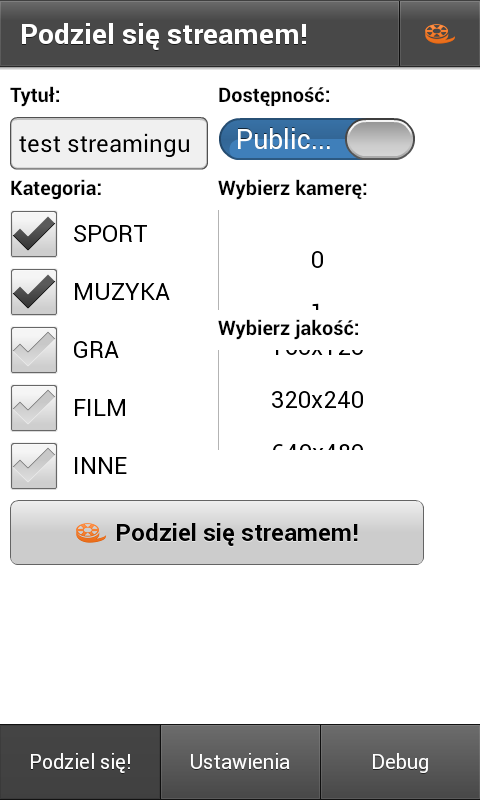
\includegraphics[width=\textwidth]{img/screens/mobile_broadcaster/panel-udostepniania-streamu.png}
        \caption{Panel udostępniania streamu.}
        \label{fig:MB1}
    \end{subfigure}
    \quad
    \begin{subfigure}{0.4\textwidth}
        \centering
        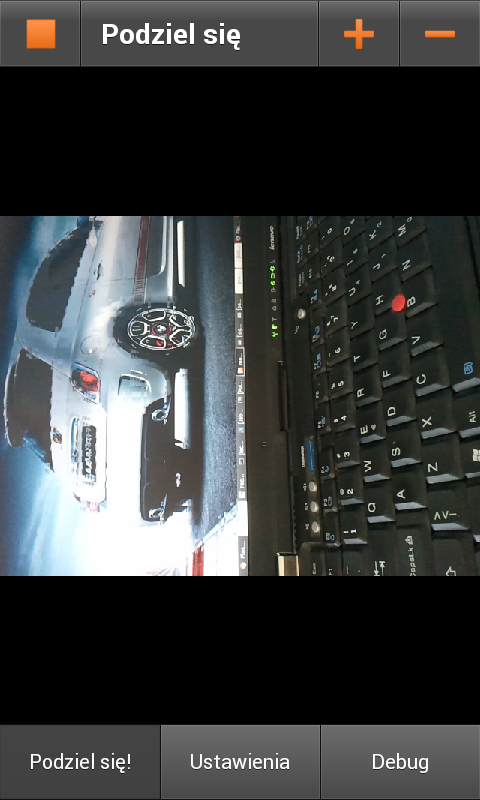
\includegraphics[width=\textwidth]{img/screens/mobile_broadcaster/streaming-wideo.png}
        \caption{Streaming wideo.}
        \label{fig:MB2}
    \end{subfigure}
    \caption{Screenshoty z Mobile Receivera część 1.}
\end{figure}

\begin{figure}[ht]
    \centering
    \begin{subfigure}{0.3\textwidth}
        \centering
        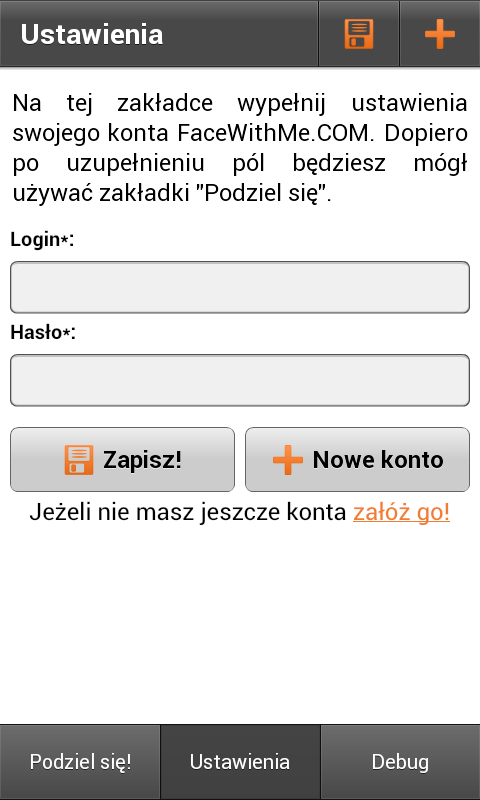
\includegraphics[width=\textwidth]{img/screens/mobile_broadcaster/panel-ustawien.png}
        \caption{Panel ustawień aplikacji.}
        \label{fig:MB3}
    \end{subfigure}
    \quad
    \begin{subfigure}{0.3\textwidth}
        \centering
        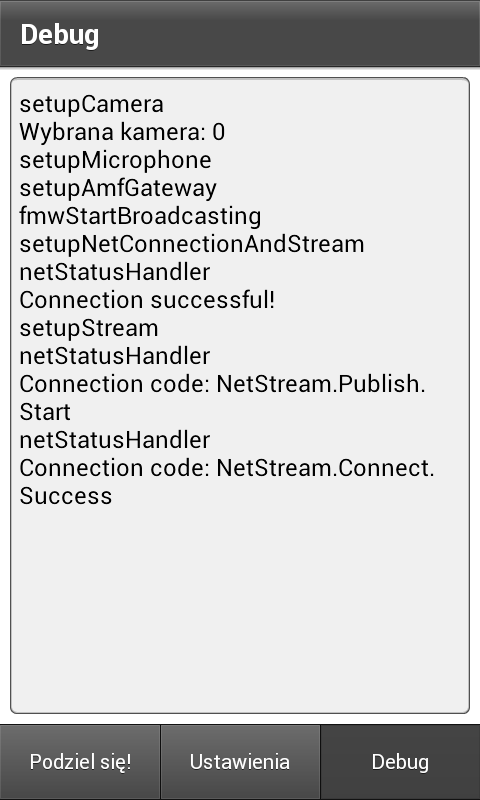
\includegraphics[width=\textwidth]{img/screens/mobile_broadcaster/panel-debug.png}
        \caption{Panel DEBUG aplikacji.}
        \label{fig:MB4}
    \end{subfigure}
    \quad
    \begin{subfigure}{0.3\textwidth}
        \centering
        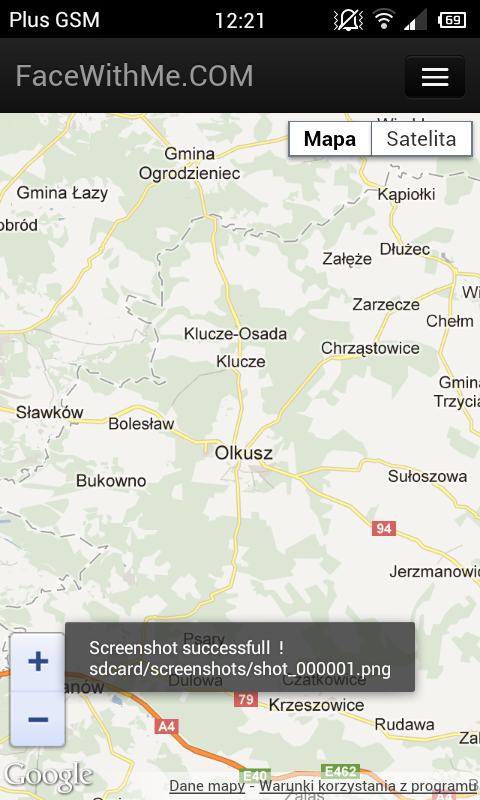
\includegraphics[width=\textwidth]{img/screens/mobile_broadcaster/interfejs-www.png}
        \caption{Interfejs WWW widoczny z poziomu przeglądarki mobilnej.}
        \label{fig:MB5}
    \end{subfigure}
    \caption{Screenshoty z Mobile Receivera część 2.}
\end{figure}

\newpage
\section{Co wymaga usprawnienia}
\label{sec:ImplementacjaPrototypuCoWymagaUsprawnienia}
Przy implementacji prototypu systemu, nie skupiano się na sprawach pobocznych jak interfejs czy komunikacja z użytkownikiem. Głównie kierowano się intencją przetestowania w praktyce działania technologii Adobe P2P Multicasting. Dlatego też system wymaga znacznej ilości poprawek zanim może zacząć być wykorzystywany publicznie. Przygotowany prototyp traktować można jako bazę wyjściową do zapoznania się z działaniem i wydajnością technologii. Główne braki prototypu systemu to:

\begin{packed_item}
    \item{Brak szyfrowania połączeń HTTP pomiędzy użytkownikiem a systemem, dotyczy także logowania.}
    \item{Brak jakiejkolwiek autoryzacji serwera RTMFP, jest dostępny publicznie.}
    \item{Brak zabezpieczenia publicznego/prywatnego streamu wideo.}
    \item{Brak całego Mobile Receivera, szczegóły \namedref{sec:EtapIwstepnaArchitekturaSystemu}.}
    \item{Brak całego Browser Broadcastera, szczegóły \namedref{sec:EtapIwstepnaArchitekturaSystemu}.}
    \item{Isnienie panelu DEBUG w Mobile Broadcasterze.}
    \item{Brak obrotu komponentu kamery względem obrócenia urządzenia w Mobile Broadcasterze co skutkuje przesuwaniem obrazu kamery góra/dół, gdy kamera fizycznie poruszana jest prawo/lewo.}
    \item{Brak automatycznego usuwania streamu z Interfejsu WWW w przypadku nieoczekiwanego przerwania działania Mobile Broadcastera.}
    \item{Brak komunikatów skierowanych do użytkownika Mobile Broadcastera, informujących o stanie lub błędach aplikacji.}
    \item{Brak wyłączania trybu czuwania urządzenia podczas udostępniania streamu.}
    \item{Brak aplikacji na iOS -- Głównym powodem dla którego nie udało się stworzyć i przetestować aplikacji na platformę iOS jest koszt licencji Apple Developer Account (99\$), jaki trzeba ponieść, aby dostać możliwość umieszczania aplikacji na Apps Market oraz testowania aplikacji na własnym telefonie (szczegóły można znaleźć \cite{UnknAuth11}). Z powodu zastosowania technologii Adobe AIR for Mobile, nie ma możliwości testowania aplikacji za pomocą XCode i wirtualnego środowiska iOS. Z tego powodu dostępność komputerów Mac na uczelni na wiele się nie zdała.}
    \item{Brak środowiska testującego oraz testów kodu źródłowego Adobe Flash Platform, zarówno kodu Adobe AIR for Mobile jak i Adobe Flash.}
\end{packed_item}

\newpage
\section{Dokumentacja}
Zgodnie z filozofią metodyki,,XP'' (szczegóły \namedref{sec:ZMTOzalozenia}), dokumentacja projektu sprowadza się do opisu architektury oraz komentarzy kodu, testów oraz komentarzy do testów. Unika się tworzenia bazy wiedzy, która najczęściej jest po pewnym czasie nieaktualizowana.

Dlatego też, aby zapoznać się z działaniem systemu należy przejrzeć architekturę systemu, a następnie zapoznać się bezpośrednio z kodem źródłowym i zawartymi w nim komentarzami.

\subsection{Uruchomienie systemu}

Aby uruchomić system z kodu źródłowego należy przygotować szereg aplikacji i skonfigurować odpowiednio środowisko. Niżej prezentowana jest lista części systemu, wraz z opisem jak daną część uruchomić.

\begin{description}
    \item[Interfejs WWW] Uruchomić aplikację Django, znajdującą się w dołączonym kodzie źródłowym w katalogu \texttt{./src/Django/facewithme/}. Wymagane do uruchomienia biblioteki środowiska Pythonowskiego w formacie pliku wymagań programu PIP znajdują się w \texttt{./src/Django/facewithme/requirements/requirements.txt}. Instrukcja instalacji i wdrożenia aplikacji Django znajduje się w \cite{DjangoDocs}. System wdrożony został przy wykorzystaniu Django 1.4.1.
    \item[Baza danych] Uruchomić i zainstalować serwer PostgreSQL (\cite{PostgreSQL}). Zainstalować rozszerzenie GIS zgodnie z instrukcją zamieszczoną w \cite{DjangoPostGIS}. System wdrożony został przy wykorzystaniu PostgreSQL 9.1.
    \item[Serwer RTMFP] Uruchomić serwer Cumulus. Instrukcja instalacji znajduje się w \cite{CumulusInstall}. Dodatkowo należy umieścić serwer na liście dostępnych serwerów w panelu administracyjnym aplikacji Django. Domyślnie, dodawane streamy losują jeden z dostępnych serwerów RTMFP. Można pokusić się o implementację algorytmu rozkładającego obciążenie bardziej równomiernie np. Round Robin.
    \item[Browser Receiver] Należy tak skonfigurować dołączanie obiektu flash, aby przekazywać informację na temat AMFGateway. Można do tego wykorzystać zmienną amfgateway dodając ją w widokach wyświetlających Browser Receiver. Domyślnie ustawiona jest na wartość \texttt{http://facewithme.com/amf/}.
    \item[Mobile Broadcaster] Należy uruchomić, zainstalować i skonfigurować środowisko Flash Develop zgodnie z tą instrukcją \cite{flashDevelopConfig}. W plikach źródłowych odnaleźć domyślną konfigurację AMFGateway (\texttt{./src/Flex/FaceWithMe Mobile/src/Main.mxml}) i poprawić ją na adres skonfigurowanego wcześniej Interfejsu WWW. Skompilować projekt oraz stworzyć odpowiednie paczki instalacyjne dla platform docelowych (Android / iOS).
\end{description}

W razie problemów z wyświetlaniem się streamu należy zapoznać się z plikiem pomocy \url{http://facewithme.com/help/}.

\subsection{Testy automatyczne}

Część Interfejsu WWW systemu posiada zalążki testów jednostkowych. Dotyczą one poprawnego wyświetlania widoków. Aby uruchomić testy, należy przejść do katalogu z z kodem źródłowym Django (\texttt{./src/Dajango/facewithme/}), a następnie uruchomić polecenie:

\lstset{language=Bash}
\begin{lstlisting}
python manage.py test core
\end{lstlisting}

O poprawnym wykonaniu testów informuje nas konsola, której wyjście zawiera:
\begin{lstlisting}
Creating test database for alias 'default'...
......
----------------------------------------------------------------------
Ran 6 tests in 0.822s

OK
Destroying test database for alias 'default'...
\end{lstlisting}

\subsection{Przeprowadzone testy}
\label{sec:EtapIprzeprowadzoneTesty}
System testowany był na kilku platformach. Niżej znajduje się lista konfiguracji systemu, w której poszczególne części nie wykazywały błędnego zachowania.

\begin{description}
    \item[Interfejs WWW z Browser Receiver] Google Chrome (21.0.1180.89) + Flash Player (11.3.31.232)/Linux; FireFox 15.0.1 + Flash Player 11.2.202.238/Linux; Google Google Chrome (21.0.1180.89) + Flash Player (11.3.31.232)/Windows 7;  FireFox 15 + Flash Player 11.2.202.238/Windows 7.
    \item[Mobile Broadcaster] Adobe AIR 3.4.0.254/Android 4.04/Samsung Galaxy S I, Adobe AIR 3.4.0.254/Android 3.2/Samsung Galaxy Tab 10.1.
\end{description}

\subsection{Bezpieczeństwo}
\label{sec:ImplementacjaPrototypuBezpieczenstwo}
Bardzo ważnym aspektem docelowego systemu powinno być bezpieczeństwo. Niżej wyszczególniono elementy prototypu systemu, które mają bezpośredni związek z bezpieczeństwem i sugerowane poprawki, które pomogą zabezpieczyć system.

\begin{packed_item}
    \item{Dzięki zastosowaniu technologii Adobe Flash Platform oraz wykorzystaniu protokołu RTMFP, transmisja danych pomiędzy Mobile Broadcasterem oraz Browser Receiverem jest szyfrowana. Szyfrowanie odbywa się za pomocą 128-bitowego klucza. Szczegółowe informacje można uzyskać w \cite{AdobeSecurity}}.
    \item{Komunikacja pomiędzy Interfejsem WWW, a Browser Receiverem oraz Mobile Receiverem, odbywająca się za pomocą AMFGateway powinna odbywać się za pomocą protokołu HTTPS, nie HTTP jak w prototypie.}
    \item{Logowanie do panelu administracyjnego oraz logowanie użytkowników powinno wykorzystywać protokół HTTPS, nie HTTP jak w prototypie.}
    \item{Sugeruje się przejście na HTTPS w każdej komunikacji nawiązywanej pomiędzy użytkownikiem, a Interfejsem WWW, nie HTTP jak w prototypie.}
    \item{Serwer RTMFP (Cumulus), nie udostępnia żadnego sposobu na autoryzację połączeń. Najprostszym sposobem na ograniczenie wykorzystania przez nieautoryzowanych użytkowników jest sprawdzanie \texttt{swfUrl} połączającego się klienta za pomocą rozszerzenia serwera wykorzystującego zdarzenie \texttt{onConnection} (szczegóły w \cite{CumulusDocs}).}
\end{packed_item}

\newpage
\section{Wydajność P2P Multicasting w Adobe Flash Platform}
\label{sec:ImplementacjaPrototypuWydajnoscP2P}
W tym rozdziale chciano poruszyć temat związany z wydajnością transmisji wideo za pomocą technologii P2P Multicasting. Kryterium jakie chcemy sprawdzać to opóźnienie transmisji wideo względem obrazu oryginalnego oraz jego płynność. Opóźnienie jest wyrażone w sekundach. Płynność określono jako jedną z poniższych możliwości.
\begin{description}
    \item[Obraz całkowicie płynny] Obraz zachowuje płynność ciągle.
    \item[Obraz płynny] Obraz od czasu do czasu wstrzymuje się, większą część czasu jest płynny.
    \item[Obraz skaczący] Obraz nie jest płynny, posiada natomiast więcej niż jedną klatkę na sekundę.
    \item[Obraz poklatkowy] Obraz nie jest całkowicie płynny, posiada mniej niż jedną klatkę na sekundę.
    \item[Obraz nieczytelny] Obraz pojawia się we fragmentach, wyświetlają się pomniejsze.
\end{description}

Środowisko testowe składa się z dwóch komputerów klientów, na których uruchomiono przeglądarkę Google Chrome i włączono Browser Receiver dla streamu udostępnianego przez Mobile Broadcaster uruchomionego na Adobe AIR 3.4.0.254/Android 3.2/Samsung Galaxy Tab 10.1. Aplikacja mobilna wysyłanie streamu wideo przeprowadza za pomocą łącza ADSL (połączenie WiFi przez router) o parametrach faktycznych 8 Mb/s pobieranie, 1 Mb/s wysyłanie danych. Alternatywnym połączeniem Mobile Broadcastera jest darmowy internet od Aero2 w technologii HSPA/HSPA+ o parametrach faktycznych 0.5 Mb/s pobieranie, 0.4 Mb/s wysyłanie danych. Komputery klienckie są połączone do tej samej sieci LAN, korzystającej z wcześniej wymienionego łącza ADSL. Test prędkości łącz został wykonany za pomocą serwisu \url{http://speedtest.net}. W poniższej tabeli znajdują się parametry łącz na których przeprowadzono testy.

\begin{table}[h]
    \centering
    \begin{tabular}{|l|l|l|l|}
        \hline
        & ping & prędkość pobierania & prędkość wysyłania \\
        \hline
        ADSL
        &
        51~ms
        &
        8~Mb/s
        &
        1~Mb/s
        \\
        \hline
        Aero2
        &
        107~ms
        &
        0.5~Mb/s
        &
        0.4~Mb/s
        \\
        \hline
    \end{tabular}
    \caption{Parametry łącz na których zostały przeprowadzone testy.}
\end{table}

Wpływ na badane kryteria mają parametry:
\begin{packed_item}
    \item{Rozdzielczość obrazu w transmisji wideo, która jest przekazywana.}
    \item{Ilość klientów uczestniczących w transmisji P2P Multicast.}
    \item{Łącze wykorzystywane przez Mobile Broadcastera.}
    \item{Łącze wykorzystywane przez Browser Receivera.}
\end{packed_item}

Tabela przedstawiająca płynność transmisji oglądanej na ekranie Browser Receivera, względem rozdzielczości przesyłanego strumienia w pikselach. Dla dwóch włączonych Browser Reveiverów, po jednej instancji per komputer klient:
\begin{table}[h]
    \centering
    \begin{tabular}{|l|l|l|l|l|}
        \hline
        & 80x60px & 160x120px & 320x240px & 640x480px \\
        \hline
        ADSL
        &
        obraz całkowicie płynny 
        &
        obraz całkowicie płynny
        &
        obraz płynny
        &
        obraz skaczący
        \\
        \hline
        Aero2
        &
        obraz płynny
        &
        obraz poklatkowy
        &
        obraz nieczytelny
        &
        obraz nieczytelny
        \\
        \hline
    \end{tabular}
    \caption{Płynność transmisji wideo w danej rozdzielczości względem wykorzystywanego łącza dla dwóch Browser Receiverów.}
\end{table}

Tabela przedstawiająca opóźnienie transmisji oglądanej na ekranie Browser Receivera, względem rozdzielczości przesyłanego strumienia w pikselach. Dla dwóch włączonych Browser Reveiverów, po jednej instancji per komputer klient:
\begin{table}[h]
    \centering
    \begin{tabular}{|l|l|l|l|l|}
        \hline
        & 80x60px & 160x120px & 320x240px & 640x480px \\
        \hline
        ADSL
        &
        opóźnienie 0s
        &
        opóźnienie 0s
        &
        opóźnienie 0,1s
        &
        opóźnienie 0-1s \\
        \hline
        Aero2
        &
        opóźnienie 0,1-0,5s
        &
        opóźnienie 2-3s
        &
        opóźnienie 4-5s
        &
        opóźnienie ~40s \\
        \hline
    \end{tabular}
    \caption{Opóźnienie transmisji wideo w danej rozdzielczości względem wykorzystywanego łącza dla dwóch Browser Receiverów.}
\end{table}

Tabela przedstawiająca płynność transmisji oglądanej na ekranie Browser Receivera, względem rozdzielczości przesyłanego strumienia w pikselach. Dla sześciu włączonych Browser Reveiverów, po trzy instancje per komputer klient:
\begin{table}[h]
    \centering
    \begin{tabular}{|l|l|l|l|l|}
        \hline
        & 80x60px & 160x120px & 320x240px & 640x480px \\
        \hline
        ADSL
        &
        obraz całkowicie płynny 
        &
        obraz płynny
        &
        obraz płynny
        &
        obraz poklatkowy
        \\
        \hline
        Aero2
        &
        obraz płynny
        &
        obraz poklatkowy
        &
        obraz poklatkowy
        &
        obraz nieczytelny
        \\
        \hline
    \end{tabular}
    \caption{Płynność transmisji wideo w danej rozdzielczości względem wykorzystywanego łącza dla sześciu Browser Receiverów.}
\end{table}

Tabela przedstawiająca opóźnienie transmisji oglądanej na ekranie Browser Receivera, względem rozdzielczości przesyłanego strumienia w pikselach. Dla sześciu włączonych Browser Reveiverów, po trzy instancje per komputer klient:
\begin{table}[h]
    \centering
    \begin{tabular}{|l|l|l|l|l|}
        \hline
        & 80x60px & 160x120px & 320x240px & 640x480px \\
        \hline
        ADSL
        &
        opóźnienie 0s
        &
        opóźnienie 0-0,3s
        &
        opóźnienie 0-0,5s
        &
        opóźnienie 0,5-2s \\
        \hline
        Aero2
        &
        opóźnienie 0-3s
        &
        opóźnienie 30s
        &
        opóźnienie 35s
        &
        opóźnienie 45s \\
        \hline
    \end{tabular}
    \caption{Opóźnienie transmisji wideo w danej rozdzielczości względem wykorzystywanego łącza dla sześciu Browser Receiverów.}
\end{table}

\newpage
%---------------------------------------------------------------------------
